\documentclass[10pt]{beamer}

\usepackage[utf8]{inputenc}
\usepackage{pgfpages}
\usepackage{dirtree}
\setbeamertemplate{note page}[plain]
\AtEndNote{\vfill \begin{center} mm:hh \end{center}}
\newcommand{\notedir}[1] {
  \note{\dirtree{#1}}}
\usepackage{tcolorbox}
\usepackage{tikz}
\usetikzlibrary{intersections,calc}
\usepackage{amsmath}
\usepackage{graphicx}
\def \heart {\textcolor{blue}{$\heartsuit$} }
\def \C {$\mathcal{C}$}





\tcbset{%
	basic/.style={colframe=black,
		      colback=white,
		      top= 0mm,
		      bottom = 2mm,
		      boxsep=0mm
		      }
}

    
\begin{document}  
    \setlength{\abovedisplayskip}{0pt}
    \setlength{\belowdisplayskip}{0pt}
    
    \beamertemplatenavigationsymbolsempty
    
    \frame{%Enoncé ex2
  
	\frametitle{Q2 Juillet 2015.}
	
	Soient $ABC$ un triangle rectangle en $A$, et $d$ une droite passant par
	$A$. On note $G$ la projection orthogonale de $B$ sur $d$, et $E$ la projection
	orthogonale de $C$ sur $d$. On note également $d_1$ la parallèle à $AC$ menée
	par $G$, et $d_2$ la parallèle à $AB$ menée par $E$. \bigskip
	\begin{itemize}
	 \item[$(a)$] Démontrer que les droites $d_1$ , $d_2$ et $BC$ sont concourantes.
	 \item[$(b)$] Déterminer le lieu géométrique du point d’intersection de $d_1$ et de
		      $d_2$ lorsque $d$ varie.
	\end{itemize}
	
	\vfill
	  
	  \pause	  
	  % Conditions
	  \begin{tcolorbox}[basic] \centering
	      	 
		      \medskip
		      \underline{Procédé} \\
		      \begin{itemize}
		       \item Repère orthonormé et équations cartésiennes,
		       \item[$(a)$] M.q. $d_1 \cap d_2 \in BC$,
		       \item[$(b)$] Point d'intersection en fonction de la pente de $d$.
		      \end{itemize}
		   		  	     
	  \end{tcolorbox}
	\notedir{%
	.1 Énoncé.
	.2 Choix : géométrie analytique.
	.3 $\Delta$ rect.~et éléments faciles à représenter dans repère..
	.4 Procédé : traduire mathématiquement ce qu'il faut démontrer..
	}  
	}
  \frame{%Résolution
	\begin{columns}[t]
		\column{.5\textwidth}\centering
		

			\underline{Dessin}\\
			
				  \begin{figure}[h]
				  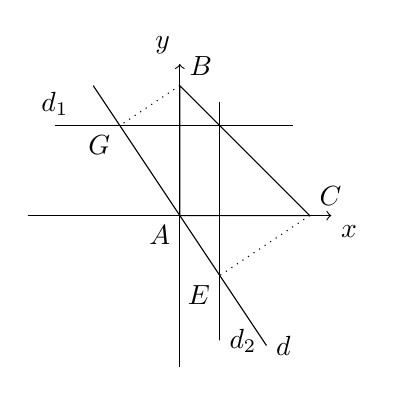
\begin{tikzpicture}[scale=0.55]
					%\draw[help lines] (-3,-3) grid (3,3); 
					
					%AXES
					\draw[->] (0,-3.5) -- (0,3.5) coordinate[label=above left:$y$]();
					\draw[->] (-3.5,0) -- (3.5,0) coordinate[label=below right:$x$]();
					%TRIANGLE
					\coordinate[label=below left:$A$] (A) at (0,0);
					\coordinate[label=above right:$B$] (B) at (0,3);
					\coordinate[label=above right:$C$] (C) at (3,0); 
					\draw (A) -- (B) -- (C) -- cycle;
					%DROITE d
					\draw[name path=d] (-2,3) -- (2,-3) coordinate[label=right:$d$];
					\path[name path=gb] (B) -- +(-3,-2);
					\path[name path=ec] (C) -- +(-3,-2);
					\path [name intersections={of=d and gb,by=G}];
					\path [name intersections={of=d and ec,by=E}];
					\draw[dotted] (B) -- (G) coordinate[label=below left:$G$]();
					\draw[dotted] (C) -- (E) coordinate[label=below left:$E$]();
					\draw (G) -- +(-1.5,0) coordinate[label=above:$d_1$]() -- +(4,0);
					\draw (E) -- +(0,-1.5) coordinate[label=right:$d_2$]() -- +(0,4);
					
					
				
				  \end{tikzpicture}
				  \end{figure}
			\begin{tcolorbox}[basic]
			\smallskip
			\centering
			\underline{Procédé} \\
		        \smallskip
		        \begin{itemize}
		       \item Repère orthonormé et équations cartésiennes,
		       \item[$(a)$] M.q. $d_1 \cap d_2 \in BC$,
		       \item[$(b)$] Point d'intersection en fonction de la pente de $d$.
		      \end{itemize}
			\end{tcolorbox}
			
		\column{.5\textwidth}\centering
		
		      \underline{Résolution} \\
		      \flushleft
		      Soit un repère orthonormé $R=(O,X,Y)$ avec : \\
		      $A (0,0), B (0,b), C (c,0)$.	\\ \bigskip	          		      		      

		      
		      \textit{Cas particulier : $d\equiv x=0$} \\ \medskip 
		      $G=B$, $E=A$.\\
		      $d_1\cap d_2=B \in BC$. \\ \bigskip

		      \textit{Cas général : $d\equiv y=mx$ ($m\in R$)}  \\ \medskip 
		      $GB\equiv y-b=-\frac{1}{m}x$, \\		    
		      $G = GB\cap d = (\frac{mb}{1+m^2},\frac{m^2b}{1+m^2})$, \\ 
		      $d_1\equiv y = \frac{m^2b}{1+m^2}$. \\ \bigskip

		      $EC\equiv y=\frac{-1}{m}(x-c)$, \\
		      $E = EC\cap d = (\frac{c}{1+m^2},\frac{mc}{1+m^2})$, \\
		      $d_2 \equiv x=\frac{c}{1+m^2}$. 
		      
	\end{columns}
  
	\notedir{%
	.1 Montrer que $d_1$, $d_2$, $BC$ sont concourantes.
	.2 Représenter éléments dans repère.
	.3 Sommets du triangle $ABC$..
	.3 Droite $d$..
	.4 Cas particulier = droite verticale.
	.5 $G$ sur $B$ et $E$ sur $A$..
	.5 $d_1$ = horizontale passant par $B$..
	.5 $d_2$ = verticale passant par $A$..
	.5 Intersection est sur $BC$ par évidence..
	.4 Cas général = équation normale d'une droite.
	.5 $G$ intersection perpendiculaire à $BC$ par $B$ et $d$..
	.5 $E$ intersection perpendiculaire à $BC$ par $C$ et $d$..
	.5 $d_1$ = horizontale passant par $B$..
	.5 $d_2$ = verticale passant par $A$..
	.5 Intersection est sur $BC$ par calcul..
	}}
	
  \frame{ 
	\begin{columns}[t]	  
	\column{.5\textwidth}\centering
	\underline{Dessin}\\
		
				  \begin{figure}[h]
				  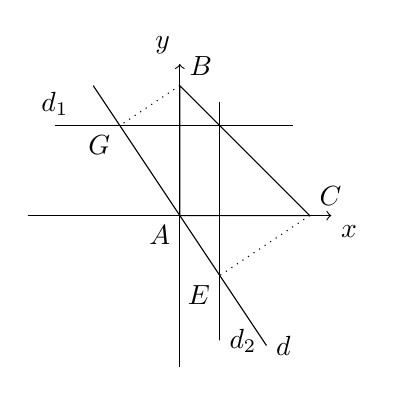
\begin{tikzpicture}[scale=0.55]
					%\draw[help lines] (-3,-3) grid (3,3); 
					
					%AXES
					\draw[->] (0,-3.5) -- (0,3.5) coordinate[label=above left:$y$]();
					\draw[->] (-3.5,0) -- (3.5,0) coordinate[label=below right:$x$]();
					%TRIANGLE
					\coordinate[label=below left:$A$] (A) at (0,0);
					\coordinate[label=above right:$B$] (B) at (0,3);
					\coordinate[label=above right:$C$] (C) at (3,0); 
					\draw (A) -- (B) -- (C) -- cycle;
					%DROITE d
					\draw[name path=d] (-2,3) -- (2,-3) coordinate[label=right:$d$];
					\path[name path=gb] (B) -- +(-3,-2);
					\path[name path=ec] (C) -- +(-3,-2);
					\path [name intersections={of=d and gb,by=G}];
					\path [name intersections={of=d and ec,by=E}];
					\draw[dotted] (B) -- (G) coordinate[label=below left:$G$]();
					\draw[dotted] (C) -- (E) coordinate[label=below left:$E$]();
					\draw (G) -- +(-1.5,0) coordinate[label=above:$d_1$]() -- +(4,0);
					\draw (E) -- +(0,-1.5) coordinate[label=right:$d_2$]() -- +(0,4);
					
					
				
				  \end{tikzpicture}
				  \end{figure}
			\begin{tcolorbox}[basic]
			\smallskip
			\centering
			\underline{Procédé} \\
		        \smallskip
		        \begin{itemize}
		       \item Repère orthonormé et équations cartésiennes,
		       \item[$(a)$] M.q. $d_1 \cap d_2 \in BC$,
		       \item[$(b)$] Point d'intersection en fonction de la pente de $d$.
		      \end{itemize}
			\end{tcolorbox}
	
	\column{.5\textwidth}\flushleft

	$d_1 \cap d_2 = (\frac{c}{1+m^2},\frac{m^2b}{1+m^2})$. \\ \medskip
	$d_1 \cap d_2\in BC \equiv \frac{x}{c} + \frac{y}{b} = 1. $ \hfill \qed (a) \\ \bigskip
	
	\centering\noindent\rule{2cm}{0.4pt}\flushleft \bigskip
	
	\textit{Cas particulier : $B (0,b)$. (1)} \\ \bigskip
	\textit{Cas général :       $\begin{cases}x= \frac{c}{1+m^2}, \\
						 y= \frac{m^2b}{1+m^2}.	 \\
				    \end{cases}$}  \\ \medskip 
		   		   
	$m^2=\frac{c}{x}-1  \rightarrow	x\in]0,c]$. \\ \medskip
	$y = -\frac{b}{c}(x-c)$. (2)\\ \bigskip \bigskip
	
	(1) et (2): \\ \medskip
	$y = -\frac{b}{c}(x-c)$, $x\in[0,c]$. \hfill \qed (b)\\ \bigskip
	
	\end{columns}
	
	\notedir{%
	.1 Suivre procédé.
	.2 Résultats du point (a).
	.3 Cas particulier.
	.4 L'intersection est le point B..
	.3 Cas général.
	.4 L'intersection est donnée par équations paramétriques.
	.5 Éliminer le paramètre.
	.6 Isoler le paramètre dans une équation..
	.6 Déduire le domaine de variation de la variable..
	.6 L'injecter dans l'autre équation.. 
	.3 Conclure avec union des 2 cas..
	}
	}
\end{document}
